\section{Vulkan initialization}

Initializing Vulkan support is quite complex due to the numerous configuration options available. 
To understand this process, we need to start with a high-level overview of a Vulkan application.
\begin{figure}[H]
    \centering
    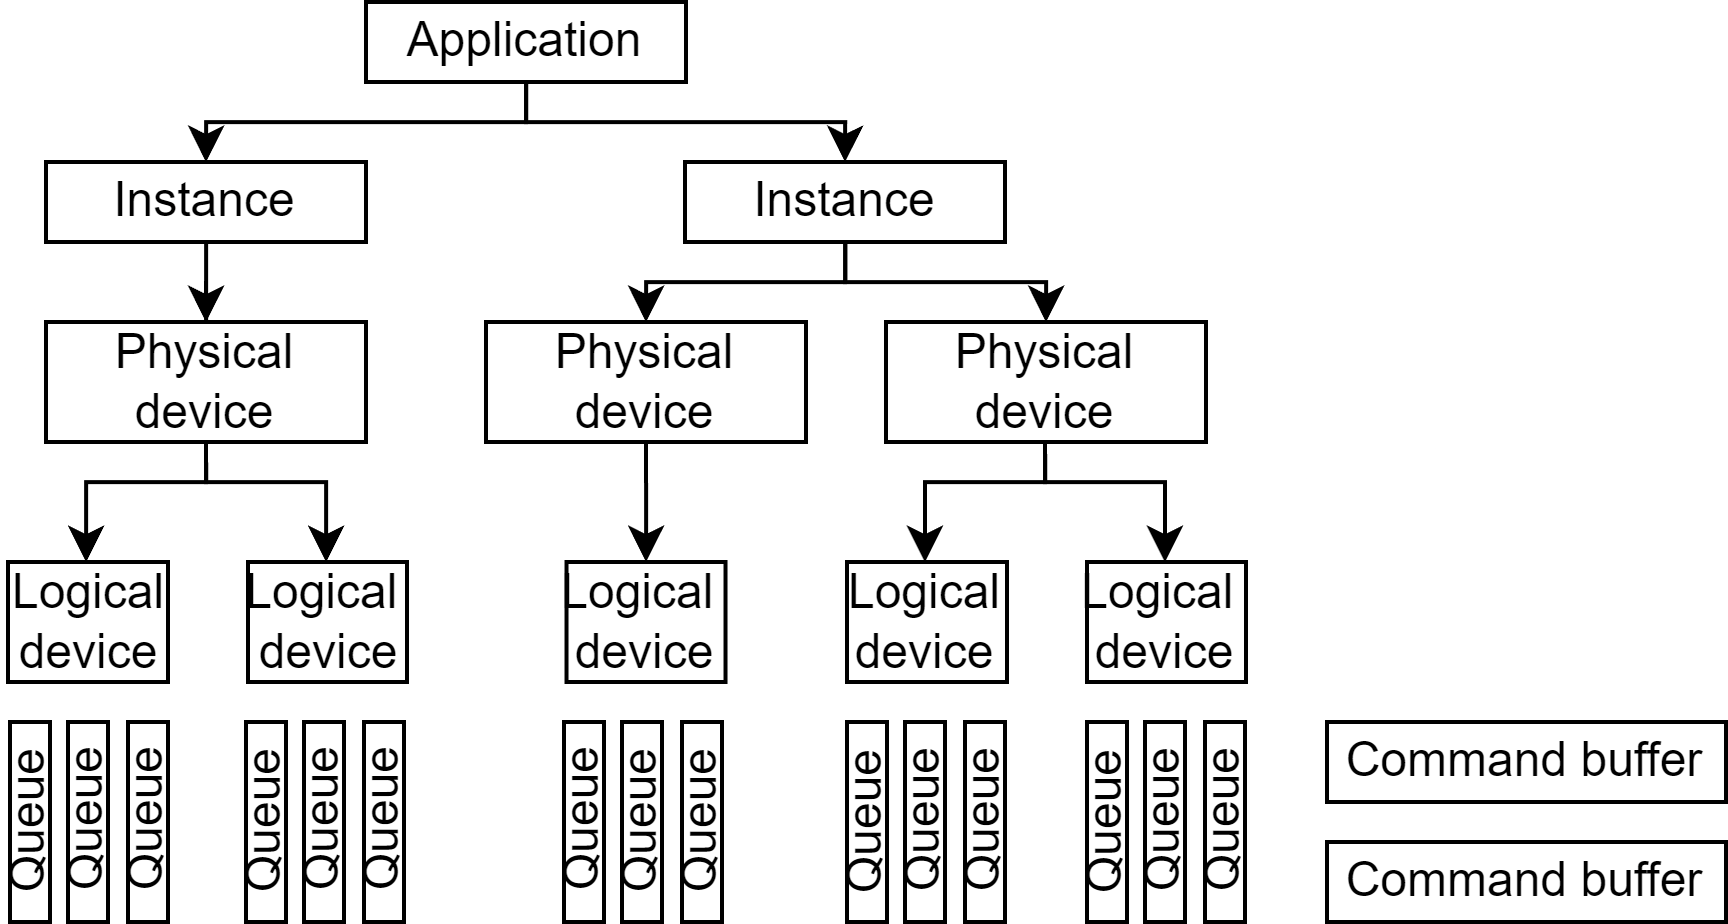
\includegraphics[width=0.4\linewidth]{images/vulkan.png}
    \caption{Vulkan architecture}
\end{figure}
At the top level, we have the Vulkan application, which can simultaneously utilize multiple software libraries that leverage Vulkan to exploit GPU capabilities. 
Each library operates independently through Vulkan instances.
\begin{itemize}
    \item \textit{Instances}: enable each software library to function independently within the application.
    \item \textit{Physical devices}: correspond to GPUs. 
        If a system has multiple GPUs, the application can use all of them in parallel to enhance performance or select the most suitable one based on power or efficiency needs.
    \item \textit{Logical devices}: allow for different configurations of the same GPU to coexist (e.g., one window with antialiasing and another without). 
        This enables the use of the same GPU for varied purposes.
\end{itemize}
To maximize parallelization, Vulkan operations are managed through queues. 
This setup allows the application to record the steps for composing the next image while the previous image's processing is still ongoing. 
Users can request multiple queues as needed and manage their synchronization to fit their application's requirements.
\begin{itemize}
    \item \textit{Queues}: facilitate parallel processing by enabling multiple tasks to be recorded and executed simultaneously.
    \item \textit{Command buffers}: store Vulkan operations and transfer them into GPU memory. 
        Each queue can handle several command buffers, allowing different threads running on separate CPU cores to record commands in parallel. 
        This approach minimizes the need to transfer data from the CPU to GPU memory, as only the necessary updates are transferred.
\end{itemize}

\subsection{Typical Vulkan application}
\begin{figure}[H]
    \centering
    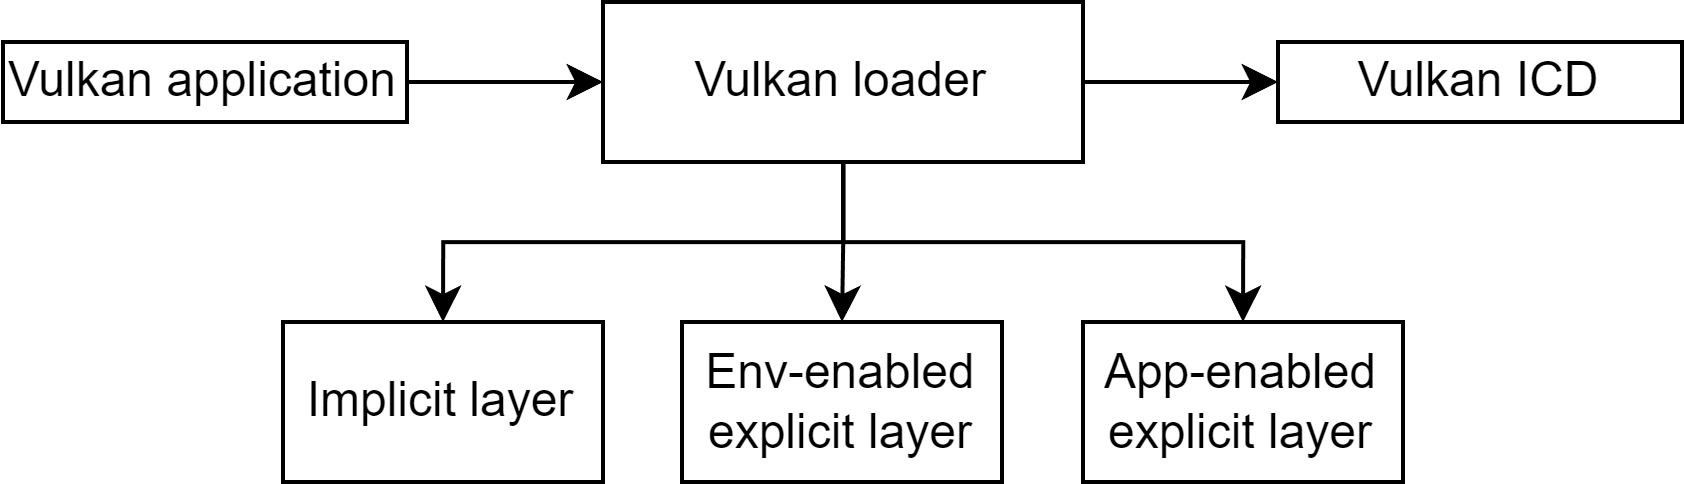
\includegraphics[width=0.4\linewidth]{images/vulkan1.png}
    \caption{Vulkan application}
\end{figure}
Most Vulkan applications, however, will use only a single library instance, operate on a single GPU, utilize just one configuration, and perform all commands in a single queue.

\paragraph*{Vulkan structure}
Vulkan's structure is inherently complex, consisting of a fixed component known as the Vulkan Loader, and a set of GPU drivers called Installable Client Devices (ICDs). 
A specific Vulkan deployment can also include a set of Extension Layers, which expose OS-specific or device-specific functions. 
These functions enable Vulkan to operate within a particular environment and access special hardware features.

\paragraph*{Instance creation}
Creating a Vulkan instance requires specifying the following information:
\begin{itemize}
    \item List of requested extensions.
    \item Name and other features of the application.
\end{itemize}
To maintain platform independence, the GLFW interface library provides the \\\texttt{glfwGetRequiredInstanceExtensions()} command, which retrieves the necessary extensions for the architecture on which the program is running.
When the instance is no longer needed, it should be released using \texttt{vkDestroyInstance()}. 
Similarly, the operating system window should be closed using \texttt{glfwDestroyWindow()}. 
To free all remaining resources, the GLFW library also requires a call to \texttt{glfwTerminate()}.

\subsection{Presentation surface}
Creating a presentation surface in Vulkan requires both a window and a Vulkan instance to be established first. 
Therefore, the presentation surface can only be created after these initial steps are completed.

The GLFW library facilitates the creation of the presentation surface through the \\\texttt{glfwCreateWindowSurface()} function. 
This function returns a handle to the surface in the VkSurfaceKHR object, which is passed as the last argument of the function.

To release the presentation surface at the end of the application, it must be destroyed before the Vulkan instance and the window are destroyed. 
This is done using the \\\texttt{vkDestroySurfaceKHR()} command.

\subsection{Physical devices}
Even though this course focuses on applications utilizing a single GPU, the system in use may have multiple GPUs available. Each physical device (GPU) is characterized by various attributes:
\begin{itemize}
    \item \textit{Properties}: includes details such as the manufacturer, whether the GPU is integrated into the CPU or separate, driver IDs, etc.
    \item \textit{Features}: indicates support for specific types of shaders, data types, graphics commands, and other capabilities.
    \item \textit{Memory types}: specifies whether the memory is shared, GPU-specific, etc.
    \item \textit{Memory heaps}: defines the total available memory.
    \item \textit{Supported queue families}: specifies the types of operations the device can perform.
\end{itemize}
Each property contains a field called limits, which indicates the maximum sizes of supported objects. 
The features structure includes numerous fields, each representing a feature that can be selected during the creation of logical devices.

\paragraph*{Memory types}
Memory types describe whether the corresponding memory is CPU-visible, GPU-only, and how it can be interfaced with Vulkan. 
Memory heaps define the available memory quantity and whether the memory is local to the GPU.

\paragraph*{Logical devices and queues}
Logical devices are created from physical devices, each containing one or more queues. 
Each physical device can support different types of queues, and the selection of a physical device may depend on the queues its logical devices can utilize.
Queues are grouped into families, each supporting different types of operations.

The function \texttt{vkGetPhysicalDeviceQueueFamilyProperties()} can enumerate the queue families supported by a physical device. 
Queue types include: graphics, compute, transfer, sparse memory management, and presentation.
A computer graphics application typically requires at least a graphics queue and a presentation queue. 
Depending on the system, these might be separate or supported by one specific queue family.

Logical devices and their queues are created using the \texttt{vkCreateDevice()} command, starting from a physical device. 
During creation, device features, extensions, and debug layers are enabled. 
Once the device is created, queue handles must be retrieved using the \texttt{vkGetDeviceQueue()} command. 
Since multiple queues per family can be created, this command requires both the family index and the queue ID.
At the end of the application, logical devices must be released.

\subsection{Command buffer}
Once queues have been retrieved, command buffers can be created to utilize them. 
Given the frequent use of multiple command buffers, they are allocated from larger groups known as command pools. 
Each command pool is specifically tied to the queue families it utilizes.

Command pools are created using the \texttt{vkCreateCommandPool()} function. 
The primary parameter to define in the creation structure is the \texttt{queueFamilyIndex} field, which specifies the queue family on which its commands will be executed. 
Command pools should be released when no longer needed using the \texttt{vkDestroyCommandPool()} function.

Command buffers are created from these pools using the \texttt{vkAllocateCommandBuffers()} function. 
Their handles are returned in \texttt{VkCommandBuffer} objects. 
The command pool handle is passed in the commandPool field of the creation structure. 
Multiple command buffers can be created in a single call; their number is specified in the commandBufferCount field.
If more than one buffer is required, the return value must be an array of the appropriate size.

Command buffers are automatically destroyed when their corresponding pool is released, eliminating the need for explicit destruction.

\subsection{Vulkan swap chain}
In Vulkan, screen synchronization is managed with a generic circular queue called the Swap Chain. 
The swap chain can handle single, double, triple buffering, and potentially longer presentation queues. 
The properties of the swap chain depend on the combination of the surface and the physical device.

Each swap chain is characterized by:
\begin{itemize}
    \item \textit{Capabilities}: basic information such as the number of buffers supported and graphical extents.
    \item \textit{Supported formats}: different color spaces and resolutions.
    \item \textit{Presentation modes}: synchronization algorithms used in Vulkan.
\end{itemize}

Swap chain capabilities provide fundamental details like the number of supported buffers and graphical extents. 
Even though colors are encoded using the RGB system, several alternative formats exist, each with different color spaces and resolutions. 
Graphics adapters can support a variety of these formats, such as 8bpc, 10bpc, and 16bpc, each offering different trade-offs between memory usage, performance, and quality. 
Swap chain formats are defined by the number of bits and components (specified in an enumeration) and the corresponding color profile.

Presentation modes, which are akin to synchronization algorithms in Vulkan terminology, are returned as an array of \\\texttt{VkPresentModeKHR} enumerations via the \\\texttt{vkGetPhysicalDeviceSurfacePresentModesKHR} command. 
Four main presentation modes are supported.

When no longer needed, swap chains can be released using the \texttt{vkDestroySwapchainKHR()} command. 
Each buffer in the swap chain is treated as a generic image in Vulkan and must be retrieved after creation.
 These images are identified by \texttt{VkImage} objects and can be retrieved using the \texttt{vkGetSwapchainImagesKHR} command.

\paragraph*{Image views}
Images can be of various formats and used for different purposes, requiring extra information about their structure and pixel access methods. 
Image views provide this necessary information by associating each image with a description of how it can be used and accessed.

After retrieving the swap chain images, their views (contained in \texttt{VkImageView} objects) must be created using the \texttt{vkCreateImageView()} command. 
The most critical information is the corresponding image, specified in the image field. Additional details will be discussed in subsequent sections.

Swap chain images are destroyed with the \texttt{VkSwapchainKHR} object, but image views must be explicitly destroyed using the \texttt{vkDestroyImageView()} command.